%%%%%%%%%%%%%%%%%%%%%%%%%%%%%%%%%%%%%%%%%
% Beamer Presentation
% LaTeX Template
% Version 1.0 (10/11/12)
%
% This template has been downloaded from:
% http://www.LaTeXTemplates.com
%
% License:
% CC BY-NC-SA 3.0 (http://creativecommons.org/licenses/by-nc-sa/3.0/)
%
%%%%%%%%%%%%%%%%%%%%%%%%%%%%%%%%%%%%%%%%%

%----------------------------------------------------------------------------------------
%	PACKAGES AND THEMES
%----------------------------------------------------------------------------------------

\documentclass{beamer}

\mode<presentation> {

% The Beamer class comes with a number of default slide themes
% which change the colors and layouts of slides. Below this is a list
% of all the themes, uncomment each in turn to see what they look like.

%\usetheme{default}
%\usetheme{AnnArbor}
%\usetheme{Antibes}
%\usetheme{Bergen}
%\usetheme{Berkeley}
%\usetheme{Berlin}
%\usetheme{Boadilla}
%\usetheme{CambridgeUS}
%\usetheme{Copenhagen}
%\usetheme{Darmstadt}
%\usetheme{Dresden}
%\usetheme{Frankfurt}
%\usetheme{Goettingen}
%\usetheme{Hannover}
%\usetheme{Ilmenau}
\usetheme{JuanLesPins}
%\usetheme{Luebeck}
%\usetheme{Madrid}
%\usetheme{Malmoe}
%\usetheme{Marburg}
%\usetheme{Montpellier}
%\usetheme{PaloAlto}
%\usetheme{Pittsburgh}
%\usetheme{Rochester}
%\usetheme{Singapore}
%\usetheme{Szeged}
%\usetheme{Warsaw}

% As well as themes, the Beamer class has a number of color themes
% for any slide theme. Uncomment each of these in turn to see how it
% changes the colors of your current slide theme.

%\usecolortheme{albatross}
%\usecolortheme{beaver}
%\usecolortheme{beetle}
%\usecolortheme{crane}
%\usecolortheme{dolphin}
%\usecolortheme{dove}
%\usecolortheme{fly}
%\usecolortheme{lily}
%\usecolortheme{orchid}
%\usecolortheme{rose}
%\usecolortheme{seagull}
%\usecolortheme{seahorse}
\usecolortheme{whale}
%\usecolortheme{wolverine}

%\setbeamertemplate{footline} % To remove the footer line in all slides uncomment this line
\setbeamertemplate{footline}[page number] % To replace the footer line in all slides with a simple slide count uncomment this line

%\setbeamertemplate{navigation symbols}{} % To remove the navigation symbols from the bottom of all slides uncomment this line
}

\usepackage{graphicx} % Allows including images
\usepackage{booktabs} % Allows the use of \toprule, \midrule and \bottomrule in tables
\usepackage{tikz}
\usepackage{babel}
%----------------------------------------------------------------------------------------
%	TITLE PAGE
%----------------------------------------------------------------------------------------

\title[SIR - Mass Tests]{SIR Model - Mass Tests} % The short title appears at the bottom of every slide, the full title is only on the title page

\author
{
  Christian Göth
  \and
  Christian Sallinger
  \and
  Florian Schager
  \and
  Paul Winkler
}
\date{\today} % Date, can be changed to a custom date

\begin{document}

\begin{frame}
\titlepage % Print the title page as the first slide
\end{frame}

\begin{frame}
\frametitle{Overview} % Table of contents slide, comment this block out to remove it
\tableofcontents % Throughout your presentation, if you choose to use \section{} and \subsection{} commands, these will automatically be printed on this slide as an overview of your presentation
\end{frame}

%----------------------------------------------------------------------------------------
%	PRESENTATION SLIDES
%----------------------------------------------------------------------------------------

%------------------------------------------------
\section{Motivation} % Sections can be created in order to organize your presentation into discrete blocks, all sections and subsections are automatically printed in the table of contents as an overview of the talk
%------------------------------------------------






\begin{frame}
\frametitle{Motivation}
\begin{itemize}
  \item Covid-19 plaguing the world
  \item Nationwide mass tests in winter
  \item Goal: reduce number of unconfirmed cases
  \item Alternative to lockdown measures
\end{itemize}
\end{frame}

%------------------------------------------------
\section{Model Description}
\begin{frame}
\frametitle{Model Description}
\begin{itemize}
\item SIR - Susceptible-Infectious-Recovered
\item Compartment Exposed: freshly infected but not yet infectious - SEIR Model
\item Split Infectious into Confirmed and Unconfirmed
\item Only Unconfirmed contribute to infections
\item Recovered people do not contribute anymore
\end{itemize}
\end{frame}

%------------------------------------------------

\section{Implementation}
\subsection{Causal Loop Diagram}
\begin{frame}
\frametitle{Causal Loop Diagram}
  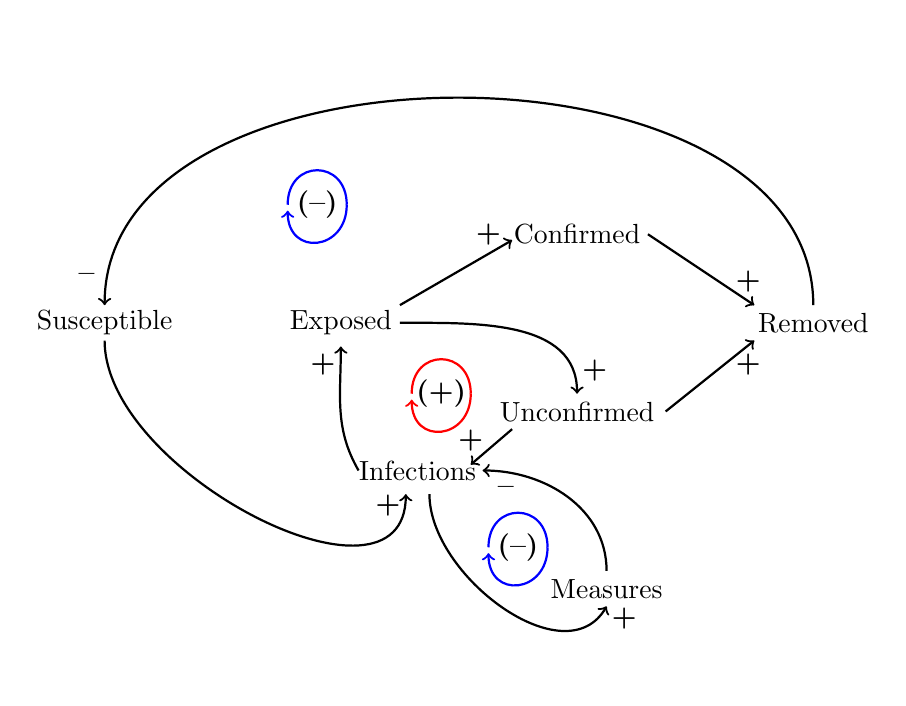
\begin{tikzpicture}[scale=0.75]
\draw[->, thick] (0.5,-2.9) to [out=-90, in=-120] (3.5,-4.8);
\draw[->, thick] (3.5,-4.2) to [out=90, in=0] (1.4,-2.5);
  \draw[->, thick] (-5,-0.3) to [out=-90, in=-90] (0.1,-2.9);
  \draw[->, thick] (0,0.3) -- (1.9,1.4);
  \draw[->, thick] (0,0) to [out=0,in=90] (3,-1.2);

  \draw[->, thick] (4.2,1.5) -- (6,0.3);
  \draw[->, thick] (4.5,-1.5) -- (6,-0.3);
\draw [->, thick] (1.9, -1.8) -- (1.2,-2.4);
 \draw [->, thick] (-0.7, -2.5) to [out=120,in=-90] (-1,-0.4);
\draw [->, thick] (7, 0.3) to [out=90,in=90] (-5,0.3);


\draw [thick, blue] (-1.9,2) to [out=90,in=90, looseness=2] (-0.9,2);
\draw [->, thick, blue] (-0.9,2) to [out=-90,in=-90, looseness=2] (-1.9,1.9);
  \node[very thick] at (-1.4,2) {\textbf{(--)}};

 \draw [thick, red] (0.2,-1.2) to [out=90,in=90, looseness=2] (1.2,-1.2);
\draw [->, thick, red] (1.2,-1.2) to [out=-90,in=-90, looseness=2] (0.2, -1.3);
  \node[very thick] at (0.7,-1.2) {\textbf{(+)}};

 \draw [thick, blue] (1.5,-3.8) to [out=90,in=90, looseness=2] (2.5,-3.8);
\draw [->, thick, blue] (2.5,-3.8) to [out=-90,in=-90, looseness=2] (1.5, -3.9);
  \node[very thick] at (2,-3.8) {\textbf{(--)}};

  \node[very thick] at (1.2,-2) {\textbf{+}};
  \node[very thick] at (1.8,-2.8) {\textbf{--}};
  \node[very thick] at (-0.2,-3.1) {\textbf{+}};
  \node[very thick] at (1.5,1.5) {\textbf{+}};
  \node[very thick] at (3.3,-0.8) {\textbf{+}};
  \node[very thick] at (5.9,0.7) {\textbf{+}};
  \node[very thick] at (5.9,-0.7) {\textbf{+}};
  \node[very thick] at (-5.3,0.8) {\textbf{--}};
  \node[very thick] at (-1.3,-0.7) {\textbf{+}};
  \node[very thick] at (3.8,-5) {\textbf{+}};
  \node[draw = none] at (-5,0) {Susceptible};
  \node[draw = none] at (-1,0) {Exposed};
  \node[draw = none] at (3,1.5) {Confirmed};
  \node[draw = none] at (3,-1.5) {Unconfirmed};
  \node[draw = none] at (7,0) {Removed};
  \node[draw = none] at (0.3,-2.5) {Infections};
  \node[draw = none] at (3.5,-4.5) {Measures};

\end{tikzpicture}


\end{frame}

%------------------------------------------------

\subsection{Stock and Flow}
\begin{frame}
\frametitle{AnyLogic Implementation}

\begin{figure}[h!]
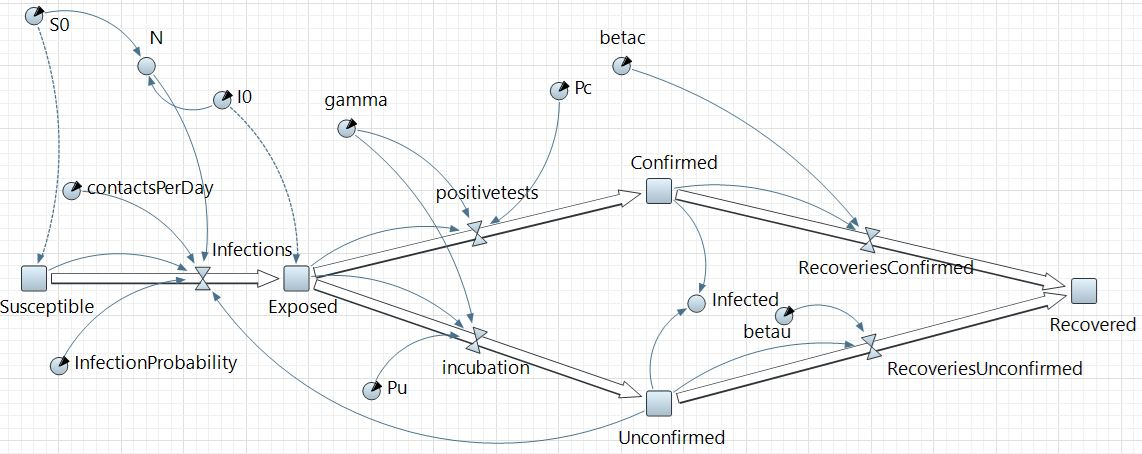
\includegraphics[width=110mm, scale = 0.5]{AnyLogicSIR}
\end{figure}
\end{frame}

%------------------------------------------------
\subsection{Parameters}
\begin{frame}
\frametitle{Parameters}
\begin{block}{$\alpha$}
  infection probability in case of contact
\end{block}

\begin{block}{c}
  contacts per day per person
\end{block}

\begin{block}{$\gamma$}
  latency rate for moving from Exposed to Confirmed or Unconfirmed
\end{block}

\begin{block}{$p_d, p_u: p_d + p_u = 1$}
  chance of being transferred to detected or undetected compartment, respecitvely
\end{block}

\begin{block}{$\beta_d, \beta_u$}
  recovery rates for detected and undetected persons
\end{block}
\end{frame}

%------------------------------------------------

\subsection{Masstests}
\begin{frame}
\frametitle{Masstests and Lockdown}
Masstests:

\begin{itemize}
  \item A portion of people move directly from the Unconfirmed to the Confirmed compartmet
  \item The flow from the Exposed compartmet is changed accordingly for the duration
  \item Occur cyclically
\end{itemize}

A lockdown occurs:
\begin{itemize}
  \item When a certain number of people are infected (Confirmed + Unconfirmed, \glqq Dunkelziffer\grqq)
  \item Lockdown measures reduce number of contacts
  \item Lift of lockdown in two steps - \glqq Lockdown light\grqq
\end{itemize}
\end{frame}


%------------------------------------------------

\subsection{}
\begin{frame}
\frametitle{Additional Assumptions}
Some assumptions were made to make a better fit with the real data:

\begin{itemize}
  \item Less cases for first lockdown
  \item Stricter first lockdown - more people follow the rules
  \item Infection-Probability lower in summer
  \item Model time: Start of Pandemic - about 1 year in the future, assuming no vaccinations!
\end{itemize}
\end{frame}

%------------------------------------------------


\begin{frame}
  \frametitle{Lockdown numbers}

  \begin{table}[!h]
  \begin{center}
  \begin{tabular}{|c||c|c|c|c|}
  \hline
    Nr. Infected &- & $\geq 45,000$ & $\leq 10,000$ & $\leq 5,000$ \\
    \hline
    contacts per Day & 14 & 2 & 6 & 9 \\
    \hline
  \end{tabular}
  \end{center}
  \caption{Numbers for first lockdown}
  \end{table}

  \begin{table}[!h]
  \begin{center}
  \begin{tabular}{|c||c|c|c|c|}
  \hline
    Nr. Infected &- & $\geq 115,000$ & $\leq 30,000$ & $\leq 20,000$ \\
    \hline
    contacts per Day & 9 & 3 & 6 & 9 \\
    \hline
  \end{tabular}
  \end{center}
  \caption{Numbers for other lockdowns}
  \end{table}

  Here the $-$ column means number of contacts per day before the respective lockdown.
\end{frame}
%------------------------------------------------

\subsection{Results}

\begin{frame}
\frametitle{Results}

\begin{table}[!h]
{\small%
\begin{center}
\begin{tabular}{|c||c|c|c|c|}
 \hline
 & 30 days    & 21 days   & 14 days  & 7 days  \\
  \hline
  \hline
      $35\%$ participation    & 199 &  170&  154  & 48   \\
  \hline
      $50\%$ participation & 174 & 151 & 91 & 11 \\
  \hline
      $70\%$ participation & 147 &  77 & 11 & 8 \\
  \hline
      $90\%$ participation & 67 &7 &7  & 6\\
      \hline
\end{tabular}
\end{center}
}%

\caption{Days of lockdown with different participation rate and interval between masstests}
\end{table}
To compare: without any masstests at all the number of days in lockdown would be $243$.
\end{frame}
%------------------------------------------------
\section{}
\begin{frame}
\Huge{\centerline{The End}}
\end{frame}

%----------------------------------------------------------------------------------------

\end{document}
